\thispagestyle{fancy}
\vspace*{40 pt}
\section{\large{\MakeUppercase{Telas IHM saída contagem}}}
 Por ser do mesmo tamanho da IHM da alimentação, foi necessário manter o mínimo de comandos possíveis e os comandos que necessitam supervisão.
 A tela principal é igual a da IHM de alimentação, por esse motivo não será descrita aqui. Também omitirei a navegação entre as telas, funcionamento de menus
 e comandos repedidos entre elas, pois são idênticos.

\subsection{Tela de comandos página 1}\label{telaComandosSaidaContagem}
\newlist {commandsInCount}{itemize}{1}
\setlist [commandsInCount]{label={}, nosep, before=\vspace{10pt}, after=\vspace{10pt}}

\begin{commandsInCount}
  \item[\ding{\dingNumber}] \textbf{Liga acionamento} - Inicia o movimento dos eixos radiais na velocidade mínima;
  \item[\ding{\dingNumber}] \textbf{JOG} - Inicia o movimento dos eixos radiais da contagem em velocidade constante;
  \item[\ding{\dingNumber}] \textbf{Desloca unidade para fora} - Desloca a unidade de contagem em direção ao LA (lado acionamento);
  \item[\ding{\dingNumber}] \textbf{Desloca unidade para dentro} - Desloca a unidade de contagem em direção ao LC (lado comando).
\end{commandsInCount}

\vspace*{\fill}
\begin{figure}[h]
  \centering
  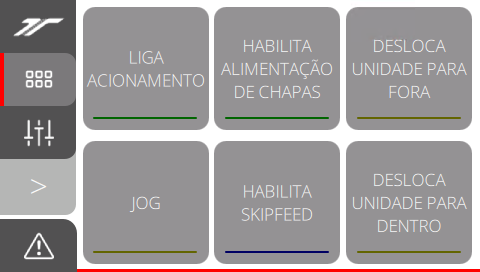
\includegraphics{src/imagesFlexo/12-IHMCNT/e-2.png}
\end{figure}
\vspace*{\fill}

\newpage
\thispagestyle{fancy}
\vspace*{40 pt}
\subsection{Tela de comandos página 2}\label{telaComandosSaidaContagem2}
  O único botão que não é repetido na tela de comandos da IHM da alimentação é o \textbf{Descarta pacote}, que descarta o pacote atual e inicia a contagem do próximo pacote.
\vspace*{\fill}
\begin{figure}[h]
  \centering
  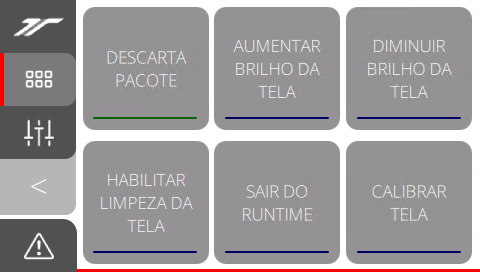
\includegraphics{src/imagesFlexo/12-IHMCNT/e-3.png}
\end{figure}
\vspace*{\fill}

\newpage
\thispagestyle{fancy}
\vspace*{40 pt}
\subsection{Tela de ajustes pagina 1}\label{telaAjustesSaidaContagem}
  A tela de ajustes é similar da IHM de alimentação, com diferença entre o JOG dos eixos, porém o principio é o mesmo. A segunda tela de ajustes é muito similar
   a da IHM de alimentação por este motivo não será descrita e nem exibida aqui.
\vspace*{\fill}
\begin{figure}[h]
  \centering
  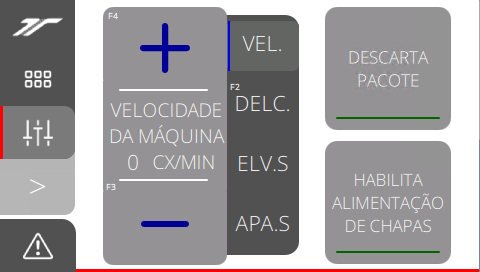
\includegraphics{src/imagesFlexo/12-IHMCNT/e-4.png}
\end{figure}
\vspace*{\fill}


